\subsection{Component Collection}
\label{subsec:detailed_component_collection}
The component collection is where all the different building blocks comes together.
It is responsible for containing a collection of a specific component type.
The collection was designed for fast contiguous processing of component groups internally within the ECS,
while supporting external lookups on individual components.

\subsubsection{Explanation}
The component collection functions like a dynamically sized pool for components of a specific type.
The following paragraphs explains the different decisions faced when creating the component collection.

\paragraph{Contiguous Byte Buffer}
Components are stored in a contiguous buffer of raw memory,
which is manually iterated over with byte pointers.
The rationale behind this is that the type of a component is opaque
to the collection, meaning it is unknown at compile time
how many bytes that is needed to increment a pointer to the next object.
Operations on the components are done by reinterpreting the components from bytes to components,
and send them as parameters to the operation types belonging to the component.
The reasoning for using a contiguous memory buffer is to make better usage of hardware caching mechanisms.

\paragraph{Reallocation \& Growth Strategy}
\label{par:detailed_component_collection_reallocation_growth}
The buffer is contiguous memory, which needs to be reallocated when new components are added.
This can be a costly operation, but is mitigated by using a simple growth strategy.
When a collection needs to reallocate it will expand the buffer size based it's growth factor.
The new size of the collection is simply its old size multiplied with its growth factor.
This leads to an amortized constant algorithmic complexity when adding a new component to the collection,
however some extra overhead is required to keep the index map in a valid state.
\todo{Ask mariusz if using the word amortized is to "complex"}

\paragraph{Lifecycle Partitioning}
The components in the collection is further grouped together and partitioned based on their stage
in the entity lifecycle\secref{subsec:high_level_lifecycle} as seen in figure \ref{fig:component_collection_partitioning}.
Pointers are used to indicate where the different partitions in the collection begin.
Transitioning components to other stages in the lifecycle therefore means to find the component,
swapping it with the the first component in a partition and increment or decrement the partition pointer.

\begin{figure}[tbp]
    \begin{center}
    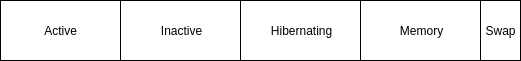
\includegraphics[scale=0.45]{images/component_collection_partitioning.png}
    \caption{Component Collection Lifecycle Partitioning}
    \label{fig:component_collection_partitioning}
    \end{center}
\end{figure}

\paragraph{Index Mapping}
Collections are often queried for their components, meaning that some form of lookup is needed.
The problem was solved by adding an indexing structure on top of the collection.
A sorted vector containing entity ids and pointers to the different components is used,
allowing for faster lookup through a binary search, as seen in figure \ref{fig:component_collection_index_map}.

\begin{figure}[tbp]
    \begin{center}
    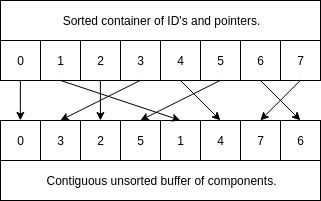
\includegraphics[scale=0.45]{images/component_collection_index_map.png}
    \caption{Component Collection Index Map}
    \label{fig:component_collection_index_map}
    \end{center}
\end{figure}

\paragraph{Iterator Invalidation}
When using contiguous memory, iterator invalidation is often a problem, and this case is no different.
After a reallocation any references to objects in the old memory location are invalidated,
and accessing them could result in undefined behavior.
This problem was solved with smart handles and generations.

\subparagraph{Generations}
A generation is a simple integer, whose value is used to indicate the number of times any action that
could have invalidated iterators within a collection has occurred, for example reallocation,
or movement of components.

\subparagraph{Smart Handles}
The smart handle is a simple structure that is handed to external users of the ECS,
it has smart pointer semantics and functions like a reference to a component while also being tolerant of iterator invalidation.
A smart handle consists of a pointer to its component, the id of the component,
a pointer to the collection the component belongs to, and lastly the generation when the smart handle was last updated.
When a smart handle is dereferenced it will look up the collection of the component and check its current generation
against its own. If the generation of the collection is newer than the generation of the handle,
an invalidation has occurred and the handle will do a search for its component before returning its pointer.
If the generation is the same the component does not need to be searched for and the pointer that the handle is currently holding is valid.

\subsubsection{Motivation for Component Collection}
The main motivation behind the component collection was a desire for contiguous memory\reqref{req:contiguous_memory}, and avoiding unnecessary
branching to check a components stage in the lifecycle.
It was also desirable to be able to move memory around internally freely, without having to worry greatly about
iterator invalidation. This was the motivation behind the smart handles, generations and index mapping, which were loosely based
on Reinalter\cite{molecular_matters_dod_external_references}'s external references functionality.

\subsubsection{Alternatives to Component Collection}
The component collection is an important part of the NOX ECS, and several alternative solutions could have been used instead.

\paragraph{Unpartitioned}
As stated earlier the components within a collection are partitioned based on their stages in the lifecycle,
this means that a lot of memory movement and pointer upkeep is happening within the collection.
An alternative could be to not partition the components. However that would mean that another way of storing
lifecycle information would be needed, for example a state variable.
It would also lead to worse branch prediction, as components would need to be queried about their state.
Avoiding partitioning would also lead to less iterator invalidation, as moving memory around would
only be needed to avoid fragmentation when removing a component.

\paragraph{Semi Contiguous Memory}
Requiring full contiguous memory might be a bit to extreme for the collection, as this leads to
reallocation in several cases. Going for a semi contiguous approach akin to that of a standard C++ deque\footnote{\url{http://en.cppreference.com/w/cpp/container/deque}},
or a linked list containing several contiguous memory segments.
Such an approach could lead to lower costs of reallocation, while still allowing for efficient use of caching mechanisms
when iterating.
Searching, removal and partitioning could suffer from such an implementation.

\paragraph{Partitioned \& Sorted}
Currently the components are partitioned, but not sorted internally within the partitions.
Soring the components internally would allow for faster look ups without the need of the index mapping.
The main reason for not implementing this was a lack of development time.

\paragraph{Lookups}
Several different approaches could have been taken for the lookup of components, rather than the index mapping solution,
these alternatives are described below.

\subparagraph{External References}
The current smart handle implementation might be more complex than necessary, and does incur a deterministic but hidden lookup\footnote{Hidden in terms that it is not clear from the syntax whether or not a lookup is needed at face value}.
A simpler solution could be to go for an external reference system like the one described by Reinalter\cite{molecular_matters_dod_external_references},
where users are given an index and generation into a sparse array, which indexes into the regular component array.
The main reason for not going with this approach was originally to not use extra space for the outer sparse arrays.
However, when the index map was introduced to allow for faster searching, that memory was needed anyway.

\subparagraph{Hashing}
Doing lookups based on hashed values was also a possibility, however this would require an efficient hashing algorithm,
which again would require more development time.

\subsubsection{Pros of Component Collection}
The main advantage of the component collection is the contiguous access to components.
Using the contiguous access together with the partitioning allows for efficient use of caching and branch prediction mechanisms.
The collection also avoids memory fragmentation and allows for memory reuse.

\subsubsection{Cons of Component Collection}
\paragraph{Memory Movement}
There is a lot of memory movement overhead required for this structure to avoid fragmentation and maintaining the partitioning, which can be quite expensive when working with types that are heavy to move.

\paragraph{Frequent Iterator Invalidation}
While the smart handles fix the problem with stale references to components, it is not cost-free.
The search for an invalid reference is an overhead, and the frequency of invalidation depends on how often insertion,
removal or transitions happen.

\paragraph{Overhead Independent of Lifecycle}
The partitioning also adds overhead to transitions in situations where a component is not relying on the lifecycle.
While it is possible to avoid the call to a lifecycle function that is not overloaded, it is still a requirement that a component is transitioned in the proper lifecycle order to maintain the partition structure of the collection.

\paragraph{Search Overhead}
Having the index map solution does incur time overhead for searching, which can be noticeable when working with
large numbers of components at a time. However, there is room for small optimizations here and there, for example, when adding components, the chance is high that the new component will have an id which is larger than the rest, meaning that it is possible to avoid the binary search in many cases.
